% !TEX root = saveliev_physics_general_course_2.tex
%!TEX TS-program = pdflatex
%!TEX encoding = UTF-8 Unicode


\chapter[CONDUCTORS IN AN ELECTRIC FIELD]{CONDUCTORS IN AN ELECTRIC \\FIELD}\label{chap:3}
\chaptermark{CONDUCTORS IN AN ELECTRIC FIELD}


\section{Equilibrium of Charges on a Conductor}\label{sec:3_1}

The carriers of a charge in a conductor are capable of moving under the action of a vanishingly small force. Therefore, the following conditions must be observed for the equilibrium of charges on a conductor:
\begin{enumerate}[1.]
    \item The strength of the field everywhere inside the conductor must be zero:
    \begin{equation}\label{eq:3_1}
        \vec{E} = 0.
    \end{equation}

    \noindent
    In acccordance with \eqn{1_41}, this signifies that the potential inside the conductor must be constant ($\varphi=\text{constant}$).

    \item The strength of the field on the surface of the conductor must be directed along a normal to the surface at every point:
    \begin{equation}\label{eq:3_2}
        \vec{E} = \vec{E}_n.
    \end{equation}

    \noindent
    Consequently, when the charges are in equilibrium, the surface of the conductor will be an equipotential one.
\end{enumerate}

If a charge $q$ is imparted to a conducting body, the charge will be distributed so as to observe conditions of equilibrium. Let us imagine an arbitrary closed surface completely confined in a body. When the charges are in equilibrium, there is no field at every point inside the conductor; therefore, the flux of the electric displacement vector through the surface vanishes. According to Gauss's theorem, the sum of the charges inside the surface will also equal zero. This holds for a surface of any dimensions arbitrarily arranged inside a conductor. Hence, in equilibrium, there can be no surplus charges anywhere inside a conductor---they will all be distributed over the surface of the conductor with a certain density $\sigma$.

Since there are no surplus charges in a conductor in the state of equilibrium, the removal of substance from a volume taken inside the conductor will have no effect whatsoever on the equilibrium arrangement of the charges. Thus, a surplus charge will be distributed on a hollow conductor in the same way as on a solid one, \ie, along its external surface. No surplus charges can be located on the surface of a cavity in the state of equilibrium. This conclusion also follows from the fact that the like elementary charges forming the given charge $q$ mutually repel one another and, consequently, tend to take up positions at the farthest distance apart.

Imagine a small cylindrical surface formed by normals to the surface of a conductor and bases of the magnitude $\deriv{S}$, one of which is inside and the other outside the conductor (\fig{3_1}). The flux of the electric displacement vector through the inner part of the surface equals zero because $\vec{E}$ and, consequently, $\vec{D}$ vanish inside the conductor. Outside the conductor in direct proximity to it, the field strength $\vec{E}$ is directed along a normal to the surface. Hence, for the side surface of the cylinder protruding outward, $D_n=0$, and for the outside base $D_n=D$ (the outside base is assumed to be very close to the surface of the conductor). Hence, the displacement flux through the surface being considered is $D\,\deriv{S}$, where $D$ is the value of the displacement in direct proximity to the surface of the conductor. The cylinder contains an extraneous charge $\sigma\,\deriv{S}$ ($\sigma$ is the charge density at the given spot on the surface of the conductor).

\begin{figure}[t]
	\begin{center}
		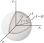
\includegraphics[scale=1]{figures/ch_03/fig_3_1.pdf}
		\caption[]{}
		\label{fig:3_1}
	\end{center}
	\vspace{-0.8cm}
\end{figure}

Applying Gauss's theorem, we get $D\,\deriv{S}=\sigma\,\deriv{S}$, \ie, $D=\sigma$. We thus see that the strength of the field near the surface of the conductor is
\begin{equation}\label{eq:3_3}
    E = \frac{\sigma}{\varepsilon_0\varepsilon}
\end{equation}

\noindent
where $\varepsilon$ is the permittivity of the medium surrounding the conductor [compare with \eqn{1_123} obtained for the case when $\varepsilon=1$].

Let us consider the field produced by the charged conductor shown in \fig{3_2}. At great distances from the conductor, equipotential surfaces have the shape of a sphere that is characteristic of a point charge (owing to the lack of space, a spherical surface is shown in the figure at a small distance from the conductor; the dash lines are field lines). As we approach the conductor, the equipotential surfaces become more and more similar to the surface of the conductor, which is an equipotential one. Near the projections, the equipotential surfaces are denser, hence, the field strength is also greater here. It thus follows that the density of the charges on the projections is especially great [see \eqn{3_3}]. We can arrive at the same conclusion by taking into account that owing to their mutual repulsion, charges tend to take up positions as far as possible from one another.

\begin{figure}[t]
	\begin{minipage}[t]{0.48\linewidth}
		\begin{center}
			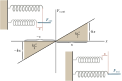
\includegraphics[scale=1]{figures/ch_03/fig_3_2.pdf}
			\caption[]{}
			\label{fig:3_2}
		\end{center}
	\end{minipage}
	\hfill{ }%space{-0.05cm}
	\begin{minipage}[t]{0.48\linewidth}
		\begin{center}
			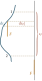
\includegraphics[scale=1]{figures/ch_03/fig_3_3.pdf}
			\caption[]{}
			\label{fig:3_3}
		\end{center}
	\end{minipage}
\vspace{-0.4cm}
\end{figure}

Near depressions in a conductor, the equipotential surfaces have a lower density (see \fig{3_3}). Accordingly,
the field strength and the density of the charges at these spots will he smaller. In general, the density of charges with a given potential of a conductor is determined by the curvature of the surface---it grows with an increase in the positive curvature (convexity) and diminishes with an increase in the negative curvature (concavity). The density of charges is especially high on sharp points. Consequently, the field strength near such points may be so great that the gas molecules surrounding the conductor become ionized. Ions of the sign opposite to that of $q$ are attracted to the conductor and neutralize its charge. Ions of the same sign as $q$ begin to move away from the conductor, carrying along neutral molecules of the gas. The result is a noticeable motion of the gas called an electric wind. The charge of the conductor diminishes, it flows off the point, as it were, and is carried away by the wind. This phenomenon is therefore called emanation of a charge from a point.

\section{A Conductor in an External Electric Field}\label{sec:3_2}

When an uncharged conductor is introduced into an electric field, the charge carriers come into motion: the positive ones in the direction of the vector $\vec{E}$, the negative ones in the opposite direction. As a result, charges of opposite signs called \textbf{induced charges} appear at the ends of the conductor (\fig{3_4}, the dash lines depict the external field lines). The field of these charges is directed oppositely to the external field. Hence, the accumulation of charges at the ends of a conductor leads to weakening of the field in it. The charge carriers will be redistributed until conditions \eqref{eq:3_1} and \eqref{eq:3_2} are observed, \ie, until the strength of the field inside the conductor vanishes and the field lines outside the conductor are perpendicular to its surface (see \fig{3_4}). Thus, a neutral conductor introduced into an electric field disrupts part of the field lines---they terminate on the negative induced charges and begin again on the positive ones.

\begin{figure}[t]
	\begin{center}
		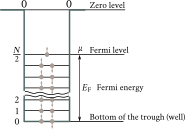
\includegraphics[scale=1]{figures/ch_03/fig_3_4.pdf}
		\caption[]{}
		\label{fig:3_4}
	\end{center}
	\vspace{-0.8cm}
\end{figure}

The induced charges distribute themselves over the outer surface of a conductor. If a conductor contains a cavity, then upon equilibrium distribution of the induced charges, the field inside it vanishes. Electrostatic shielding is based on this phenomenon. If an instrument is to be protected from the action of external fields, it is surrounded by a conducting screen. The external field is compensated inside the screen by the induced charges appearing on its surface. Such a screen also functions quite well if it is made not solid, but in the form of a dense network.

\section{Capacitance}\label{sec:3_3}

A charge $q$ imparted to a conductor distributes itself over its surface so that the strength of the field inside the conductor vanishes. Such a distribution is the only possible one. Therefore, if we impart to a conductor already carrying the charge $q$ another charge of the same magnitude, then the second charge must distribute itself over the conductor in exactly the same way as the first one. Otherwise, the charge will set up in the conductor a field differing from zero. We must note that this holds only for a conductor remote from other bodies (an isolated conductor). If other bodies are near the conductor, the imparting to the latter of a new portion of charge will produce either a change in the polarization of these bodies or a change in the induced charges on them. As a result, similarity in the distribution of different portions of the charge will be violated.

Thus, charges differing in magnitude distribute themselves on an isolated conductor in a similar way (the ratio of the densities of the charge at two arbitrary points on the surface of the conductor with any magnitude of the charge will be the same). It thus follows that the potential of an isolated conductor is proportional to the charge on it. Indeed, an increase in the charge a certain number of times leads to an increase in the strength of the field at every point of the space surrounding the conductor the same number of times. Accordingly, the work needed for transferring a unit charge from infinity to the surface of a conductor, \ie, the potential of the conductor, grows the same number of times. Thus, for an isolated conductor
\begin{equation}\label{eq:3_4}
    q = C \varphi.
\end{equation}

\noindent
The constant of proportionality $C$ between the potential and the charge is called the \textbf{capacitance}. From \eqn{3_4}, we get
\begin{equation}\label{eq:3_5}
    C = \frac{q}{\varphi}.
\end{equation}

\noindent
In accordance with \eqn{3_5}, the capacitance numerically equals the charge which when imparted to a conductor increases its potential by unity.

Let us calculate the potential of a charged sphere of radius $R$. The potential difference and the field strength are related by \eqn{1_45}. We can therefore find the potential of the sphere $\varphi$ by integrating \eqn{2_41} over $r$ from $R$ to $\infty$ (we assume that the potential at infinity equals zero):
\begin{equation}\label{eq:3_6}
    \varphi = \frac{1}{4\pi\varepsilon_0} \int_0^{\infty} \frac{q}{\varepsilon r^2}\, \deriv{r} = \frac{1}{4\pi\varepsilon_0} \frac{q}{\varepsilon R}.
\end{equation}

\noindent
Comparing Eqs. \eqref{eq:3_5} and \eqref{eq:3_6}, we find that the capacitance of an isolated sphere of radius $R$ immersed in a homogeneous infinite dielectric of permittivity $\varepsilon$ is
\begin{equation}\label{eq:3_7}
    C = 4\pi\varepsilon_0 \varepsilon R.
\end{equation}

The unit of capacitance is the capacitance of a conductor whose potential changes by \SI{1}{\volt} when a charge of \SI{1}{\coulomb} is imparted to it. This unit of capacitance is called the \textbf{farad} (\si{\faraday}).
In the Gaussian system, the formula for the capacitance of an isolated sphere has the form
\begin{equation}\label{eq:3_8}
    C = \varepsilon R.
\end{equation}

\noindent
Since $\varepsilon$ is a dimensionless quantity, the capacitance determined by \eqn{3_8} has the dimension of length. The unit of capacitance is the capacitance of an isolated sphere with a radius of \SI{1}{\centi\metre} in a vacuum. This unit of capacitance is called the \textbf{centimetre}. According to \eqn{3_5},
\begin{equation}\label{eq:3_9}
    \SI{1}{\faraday} = \frac{\SI{1}{\coulomb}}{\SI{1}{\volt}} = \frac{\num{3e9}{\cgse{C}}}{1/300} = \SI{9e11}{\centi\metre}.
\end{equation}

An isolated sphere having a radius of \SI{9e11}{\centi\metre}, \ie, a radius $1500$ times greater than that of the Earth, would have a capacitance of \SI{1}{\faraday}. We can thus see that the farad is a very great unit. For this reason, submultiples of a farad are used in practice---the millifarad (\si{\milli\faraday}), the microfarad (\si{\micro\faraday}), the nanofarad (\si{\nano\faraday}), and the picofarad (\si{\pico\faraday}) (see Vol. I, Table 3.1).

\section{Capacitors}\label{sec:3_4}

Isolated conductors have a small capacitance. Even a sphere of the Earth's size has a capacitance of only \SI{700}{\micro\faraday}. Devices are needed in practice, however, that with a low potential relative to the surrounding bodies would accumulate charges of an appreciable magnitude (\ie, would have a high charge ``capacity''). Such devices, called \textbf{capacitors}, are based on the fact that the capacitance of a conductor grows when other bodies are brought close to it. This is due to the circumstance that under the action of the field set up by the charged conductor, induced (on a conductor) or bound (on a dielectric) charges appear on the body brought up to it. Charges of the sign opposite to that of the charge $q$ of the conductor will be closer to the conductor than charges of the same sign as $q$ and, consequently, will have a greater influence on its potential. Therefore, when a body is brought close to a charged conductor, the potential of the latter diminishes in absolute value. According to \eqn{3_5}, this signifies an increase in the capacitance of the conductor.

Capacitors are made in the form of two conductors placed close to each other. The conductors forming a capacitor are called its \textbf{plates}. To prevent external bodies from influencing the capacitance of a capacitor, the plates are shaped and arranged relative to each other so that the field set up by the charges accumulating on them is concentrated inside the capacitor. This condition is satisfied (see \sect{1_14}) by two plates arranged close to each other, two coaxial cylinders, and two concentric spheres. Accordingly, parallel-plate (plane), cylindrical, and spherical capacitors are encountered. Since the field is confined inside a capacitor, the electric displacement lines begin on one plate and terminate on the other. Consequently, the extraneous charges produced on the plates have the same magnitude and are opposite in sign.

The basic characteristic of a capacitor is its capacitance, by which is meant a quantity proportional to the charge $q$ and inversely proportional to the potential difference between the plates:
\begin{equation}\label{eq:3_10}
    C = \frac{q}{\varphi_1 - \varphi_2}.
\end{equation}

The potential difference $\varphi_1-\varphi_2$ is called the \textbf{voltage} across the relevant points\footnote{A more general definition of the quantity called voltage will be given in \sect{5_3} [see \eqn{5_18}].}. We shall use the symbol $U$ to designate the voltage. Hence, \eqn{3_10} can be written as follows:
\begin{equation}\label{eq:3_11}
    C = \frac{q}{U}.
\end{equation}

\noindent
Here, $U$ is the voltage across the plates.

The capacitance of capacitors is measured in the same units as that of isolated conductors (see the preceding section).

The magnitude of the capacitance is determined by the geometry of the capacitor (the shape and dimensions of the plates and their separation distance), and also by the dielectric properties of the medium filling the space between the plates. Let us find the equation for the capacitance of a parallel-plate capacitor. If the area of a plate is $S$ and the charge on it is $q$, then the strength of the field between the plates is
\begin{equation*}
    E = \frac{\sigma}{\varepsilon_0 \varepsilon} = \frac{q}{\varepsilon_0 \varepsilon S}
\end{equation*}

\noindent
[see Eqs. \eqref{eq:1_121} and \eqref{eq:2_33}; $\varepsilon$ is the permittivity of the medium filling the gap between the plates].

In accordance with \eqn{1_45}, the potential difference between the plates is
\begin{equation*}
    \varphi_1 - \varphi_2 = E d = \frac{q d}{\varepsilon_0 \varepsilon S}.
\end{equation*}

\noindent
Hence, for the capacitance of a parallel-plate capacitor, we get
\begin{equation}\label{eq:3_12}
    C = \frac{\varepsilon_0 \varepsilon S}{d}
\end{equation}

\noindent
where $S$ is the area of a plate, $d$ is the separation distance of the plates, and $\varepsilon$ is the permittivity of the substance filling the gap.

It must be noted that the accuracy of determining the capacitance of a real parallel-plate capacitor by \eqn{3_12} is the greater, the smaller is the separation distance $d$ in comparison with the linear dimensions of the plates.

It can be seen from \eqn{3_12} that the dimension of the electric constant $\varepsilon_0$ equals the dimension of capacitance divided by that of length. Accordingly, $\varepsilon_0$ is measured in farads per metre [see \eqn{1_12}].

If we disregard the dispersion of the field near the plate edges, we can easily obtain the following equation for the capacitance of a cylindrical capacitor:
\begin{equation}\label{eq:3_13}
    C = \frac{2\pi\varepsilon_0\varepsilon l}{\ln\parenthesis{\dfrac{R_2}{R_1}}}
\end{equation}

\noindent
where $l$ is length of the capacitor, $R_1$ and $R_2$ the radii of the internal and external plates.

The accuracy of determining the capacitance of a real capacitor by \eqn{3_13} is the greater, the smaller is the separation distance of the plates $d=R_2-R_1$ in comparison with $l$ and $R_1$.

The capacitance of a spherical capacitor is
\begin{equation}\label{eq:3_14}
    C = 4\pi\varepsilon_0\varepsilon \parenthesis{\frac{R_1 R_2}{R_2 - R_1}}
\end{equation}

\noindent
where $R_1$ and $R_2$ are the radii of the internal and external plates.

Apart from the capacitance, every capacitor is characterized by the maximum voltage $\ab{U}{max}$ that may be applied across its plates without the danger of a breakdown. When this voltage is exceeded, a spark jumps across the space between the plates. The result is destruction of the dielectric and failure of the capacitor.
